% !TEX root =  main.tex
\chapter{Previous Published Results}

\section{SPP 2025 [1]: Lag Time in Diffusion Coefficient Estimation}
\label{appendix:pb30}

Section~\ref{sec:langevin-damping} introduced the Langevin damping parameter $\tau_{\text{damp}}$ and the requirement that the sampling time interval $\tau$ satisfy $\tau \gg \tau_{\text{damp}}$ before a measured diffusion coefficient can be trusted. This requirement, used throughout Chapter~3 to validate pure Brownian dynamics before any detection statistics were computed, was established in our earlier conference paper \cite{balejado2025}, which compared the mean-squared-displacement method ($D_{\text{MSD}}$) against the displacement-variance method ($D_{\text{var}}$) for polystyrene probes across a wide sweep of sampling intervals.

\begin{figure}[H]
    \centering
    \subfigure[Runtime duration: 1 million time steps\label{fig:3a}]{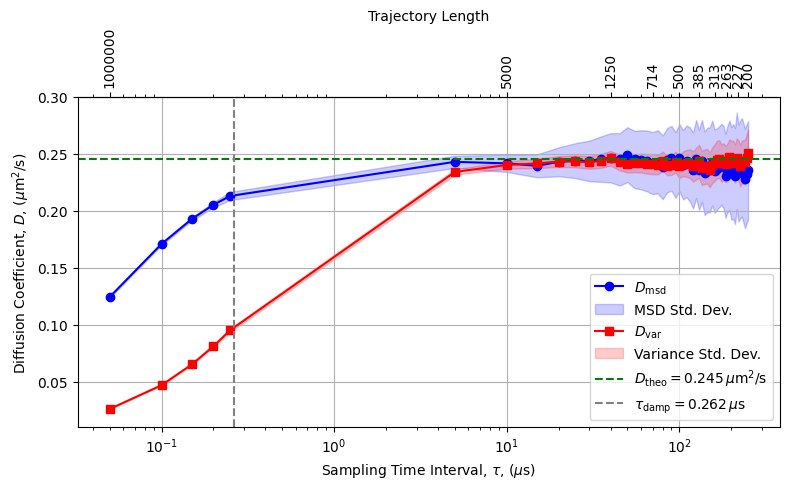
\includegraphics[width=0.45\textwidth]{figures/1mil.png}}
    \hspace{0.02\textwidth}
    \subfigure[Runtime duration: 5 million time steps\label{fig:3b}]{
    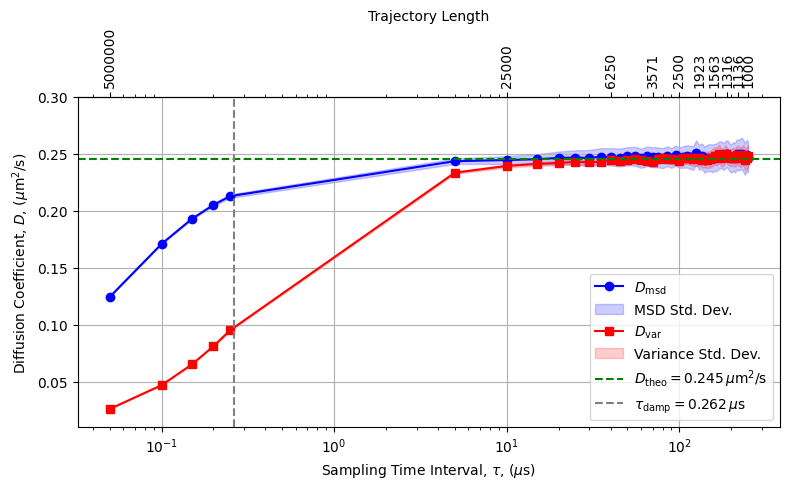
\includegraphics[width=0.45\textwidth]{figures/5mil.png}}
    \caption{$D_{\text{MSD}}$ and $D_{\text{var}}$ versus increasing sampling time interval $\tau$, from $25\,\mu\text{s}$ to $250\,\mu\text{s}$, for two total runtime durations. The green dashed line marks the theoretical Stokes-Einstein value $D_{\text{th}} = 0.245\,\mu\text{m}^2/\text{s}$; the gray dotted line marks $\tau_{\text{damp}} = 0.262\,\mu\text{s}$. Reproduced from \cite{balejado2025}.}
    \label{fig:appendix-pb30-fig3}
\end{figure}

Figure~\ref{fig:appendix-pb30-fig3} shows that both estimators underestimate $D$ when $\tau \le \tau_{\text{damp}}$, since the observed trajectory is still dominated by the ballistic, momentum-conserving regime rather than diffusive motion. Both methods converge toward $D_\text{th}$ once $\tau$ exceeds $\tau_\text{damp}$, with $D_\text{MSD}$ converging faster but $D_\text{var}$ retaining tighter precision at longer lag times, where the usable trajectory is shorter. This is the direct justification for the $\tau = 1.0\,\mu\text{s}$ sampling interval adopted throughout the present thesis (Section~\ref{sec:verifying-bm}), which sits safely inside the accurate-and-precise window identified here. 

\section{SPP 2026 [2]: Optimal Probe Density for Brownian First-Passage Detection}
\label{appendix:pa04}

Section~\ref{sec:study-gap} identified the open question this thesis answers in full. The question being whether a caldera-shaped minimum in $\langle T \rangle$ exists across probe density, and whether the ergodic product $E$ can flag the crowding transition earlier than $\langle T \rangle$ itself. That question was first posed, in preliminary form and for a single system size ($N_\text{total} = 100$), in our conference paper \cite{Balejado2026}.

\begin{figure}[b!]
    \centering
    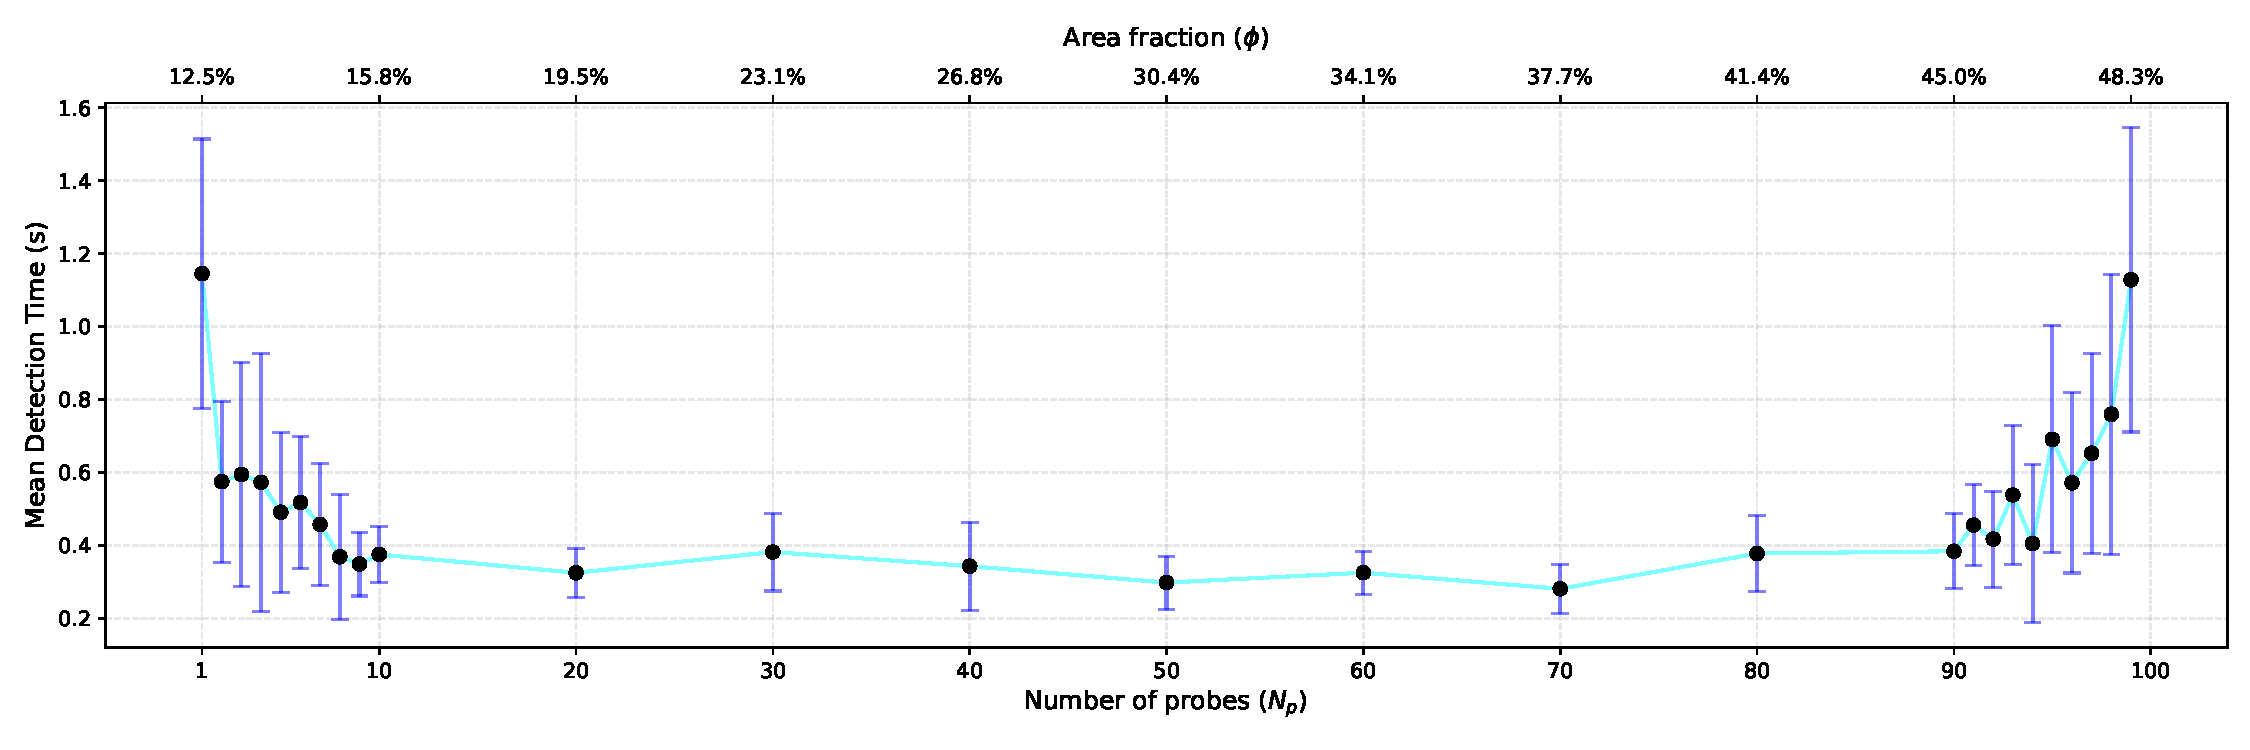
\includegraphics[width=\linewidth]{figures/Detection.pdf}
    \caption{Mean first-passage detection time $\langle T \rangle$ as a function of probe number $N_p$ for a single system of $N_{\text{total}} = 100$ particles. Error bars represent the standard deviation across 10 independent simulation seeds; the top axis shows the corresponding area fraction $\phi$. Reproduced from
    \cite{Balejado2026}.}
    \label{fig:appendix-pa04-fig1}
\end{figure}

Figure~\ref{fig:appendix-pa04-fig1} the same qualitative caldera shape reported in chapter~4 of this thesis: $\langle T \rangle$ falls from $\approx 1.15\,\text{s}$ at $N_p = 1$ at $N_p = 1$ to a minimum of $\approx 0.28\,\text{s}$ near $N_p = 70$ ($\phi \approx 37.7\,\%$), before rising again beyond $N_p \approx 80$-$90$ ($\phi \gtrsim 41$-$45\,\%$) as excluded-volume crowding sets in. This single-system result is consistent with the $N_\text{total} = 100$ system reported in Section~\ref{sec:caldera-fit} (Figure~4.5), whose fitted optimum of $N_p = 48.5$ ($\phi^* \approx 29.9\,\%$) is somewhat lower than the value read directly from the raw minimum in the conference paper, a difference attributable to the caldera model's weighted nonlinear fit smoothing over the noisier, coarser-sampled points near $N_p \approx 90$-$99$ in the original study. The present thesis extends this preliminary observation of a single-system into a systematic sweep over six system sizes and adds the ergodic product $E(N_p)$ and violin-plot distribution diagnostics to the added system sizes to independently confirm and refine the transition.  

\section{Brownian validation LAMMPS code}
{\small
\begin{verbatim}
# Initialization
units si
dimension 2
atom_style sphere

# Box
boundary p p p
region box block 0 5e-6 0 5e-6 -0.001 0.001 units box
create_box 1 box

# Single Particle
create_atoms 1 single 2.5e-6 2.5e-6 0

# Particle Mass
variable density equal 1050
variable radius equal 1e-6  # change to 0.5e-6 for foreign particle
variable volume equal (4/3.0)*3.14159*${radius}^3
variable mass equal ${density}*${volume}
set atom 1 mass ${mass}

# Particle Diameter
set atom 1 diameter 2e-6  # 2 micron diameter

# Dummy Pair Style
pair_style none

fix 1 all langevin 298 298 2.62e-7 78916 # change 2.62e-7 to 1e-7 for foreign

fix 2 all nve/sphere
fix enforce2d all enforce2d

# for computing displacement
compute myDisplacement all displace/atom

# Dump
dump 100 all custom 100 dump.100 id type x y 
\ z vx vy c_myDisplacement[1] c_myDisplacement[2]

thermo 100
timestep 5.00E-08
run 1000000
\end{verbatim}
}

\section{Impurity detection LAMMPS simulation code}
{\small
\begin{verbatim}
# Loop settings

variable Ntotal equal 100 # system_sizes : {10, 30, 50, 70, 100, 200}
variable Lf equal 2.54e-5
#  box sizes: {08.03um, 13.91um, 17.96um , 21.25um, 25.40um, 35.92um}
# seed - depends on how many trials to do
variable seed index 11111, 22222, 33333, 44444, 55555

label loop_seed
  # percentage of probe in the system size
  variable probe_percent index 0.1, 0.2, 0.3, 0.4, 0.5, 0.6, 0.7, 0.8, 0.9, 0.99 
  label loop_percent 
  variable Np_temp equal round(${Ntotal}*${probe_percent})
  if "${Np_temp} < 1" & 
  then "variable Nprobe equal 1" else "variable Nprobe equal ${Np_temp}"
  variable Nmeth equal ${Ntotal}-${Nprobe}

label loop_time
variable run_prod index 10000000 # simulation runtime: 100 mil timesteps = 1 seconds

# Intialization of the system
clear
units si
dimension 2
atom_style sphere
boundary p p p
thermo 1000

# Defining  the Box
variable expand equal 4.0
variable Li equal ${expand}*${Lf}
region box block 0 ${Li} 0 ${Li} -1e-6 1e-6 units box
create_box 2 box

# Particle parameters
variable rho equal 1050.0
variable r equal 1.0e-6
variable d_probe equal 2.0e-6
variable d_meth equal 1.0e-6
variable m equal ${rho}*(4.0/3.0)*PI*${r}^3

# Creating the particles
variable seed_meth equal ${seed}+9876
create_atoms 1 random ${Nprobe} ${seed} box
create_atoms 2 random ${Nmeth}  ${seed_meth} box

set type 1 mass ${m}
set type 2 mass ${m}
set type 1 diameter ${d_probe}
set type 2 diameter ${d_meth}

group probe type 1
group meth  type 2

velocity all set 0.0 0.0 0.0

neighbor 3.0e-6 bin
neigh_modify delay 0 every 1 check yes

# 3 Stage simulation to ensure reliable diffusion
# Optional: First dump - overall dump
# dump dbg all custom 5000 dump_debug_Np${Nprobe}_seed${seed} id type x y vx vy
# dump_modify dbg sort id

# STAGE 1: OVERLAP REMOVAL (SOFT, OVERDAMPED)
timestep 5.0e-8
pair_style soft 3.0e-6
pair_coeff * * 50.0
fix relax all langevin 298 298 1.0e-6 ${seed}
fix lim all nve/limit 1.0e-8
fix e2d all enforce2d
run 50000
unfix relax
unfix lim
unfix e2d

# STAGE 2: COMPRESSION (STILL SOFT)
fix comp all deform 1 x final 0 ${Lf} y final 0 ${Lf} units box remap x
fix relax2 all langevin 298 298 1.0e-6 ${seed}
fix lim2 all nve/limit 1.0e-8
fix e2d2 all enforce2d
run 100000
unfix comp
unfix relax2
unfix lim2
unfix e2d2

# STAGE 3: WCA + BROWNIAN PRODUCTION
timestep 1.0e-8
variable methprobe equal (${d_probe}+${d_meth})/2
variable denominator equal 1.122462

variable sigma11 equal ${d_probe}/${denominator}
variable sigma22 equal ${d_meth}/${denominator}
variable sigma12 equal ${methprobe}/${denominator}
variable rc11 equal 1.122462*${sigma11}
variable rc22 equal 1.122462*${sigma22}
variable rc12 equal 1.122462*${sigma12}

variable ljcut equal ${rc12}
pair_style lj/cut ${ljcut}
pair_modify shift yes
pair_coeff 1 1 1.0e-21 ${sigma11} ${rc11}
pair_coeff 2 2 1.0e-21 ${sigma22} ${rc22}
pair_coeff 1 2 1.0e-21 ${sigma12} ${rc12}

variable seed2 equal ${seed}+12345
fix brown1 probe langevin 298 298 2.62e-7 ${seed} 
fix brown2 meth langevin 298 298 1e-7 ${seed2} 
fix int all nve
fix e2d3 all enforce2d

compute disp all displace/atom
dump prod all custom 100 dump_Ntot${Ntotal}_Np${Nprobe}_Nm${Nmeth}_seed${seed} id type x y
dump_modify prod sort id

run ${run_prod}

#CLEANUP
unfix brown1 
unfix brown2
unfix int
unfix e2d3
undump prod 

# loop Control
  next probe_percent
  jump SELF loop_percent

next seed
jump SELF loop_seed
\end{verbatim}
}















% \hspace{\parindent} You don't need to worry about equations within
% the appendix since \LaTeX automatically formats the equation
% numbers for you. For example,
% \begin{equation}\label{eq:appendixEqn}
%     c^2 = a^2 + b^2
% \end{equation}
% becomes the Pythagorian theorem where $c$ is the length of the
% longest side of any right triangle.

% \section{Codes as appendix}

% \hspace{\parindent}Include your codes when necessary to your
% thesis/dissertation. To do this, you may use \verb+verbatim+
% environment as follows. \textbf{WARNING:} All verbatim and
% verbatiminput environments should always be treated as a separate
% paragraph.  When included in a text paragraph, it sometimes happen
% to reduce the 1.5 spacing to the usual single-spaced text.

% {\small
% \begin{verbatim}
%  #include <iostream>
%  using std::cout;
%  using std::endl;

%  int main( void )
%  {
%     cout << "Hello world!" << endl;
%     return 0;
%  }
% \end{verbatim}
% }

% The \verb+{\small }+ bracketed region is used to lower the font
% size of the entire verbatim text.  This will save you much space
% and give a more aesthetical look in your manuscript.

% On the other hand, when very long codes are wished to be included
% automatically without the tedious cut and paste procedure, you may
% include them using the \verb+\verbatiminput+ command as follows.
% You may want to include a short description of the code of course.

% {\small
%  \verbatiminput{"codes/newC.cpp"}
% }

% This time, you may just include your recent codes by just
% copy-paste-ing the codes (as long they are clean!) into the
% directory \verb$codes/$ in the directory where this file is saved.
